\chapter{Percobaan Awal}
\label{chap:percobaan_awal}
Pada bab ini akan dijelaskan analisis masalah penelitian ini. Analisis meliputi Eksplorasi Teknologi, Dataset Pada HTTP Archive, Langkah-Langkah Query Yang Dilakukan.

\section{Eksplorasi Teknologi}
\subsection{BigQuery}
Dalam pengerjaan skripsi ini akan menggunakan teknologi bernama BigQuery. Di dalam BigQuery, terdapat salah satu fitur yang akan digunakan yaitu membuat dataset baru. Dataset bisa saja diambil dari public dataset maupun membuat sendiri datasettersbut. Dataset berisi tabel-tabel yang akan dianalisis. Tabel-tabel tersebut dapat dibuat secara manual maupun di-\textit{upload}.

Berikut ini langkah-langkah dalam pembuatan dataset dan tabel:
\begin{enumerate}
	\item Membuka \href{https://console.cloud.google.com/getting-started}{Google Cloud Project Page}.
	\begin{figure}[H]
		\centering  
		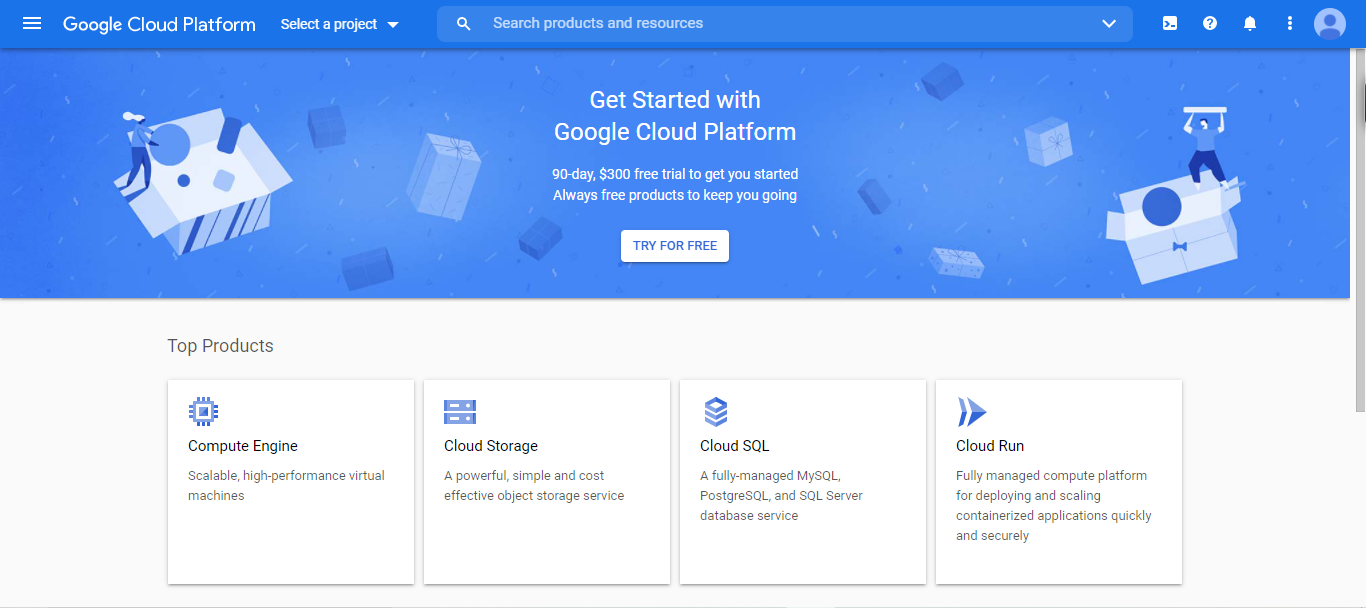
\includegraphics[scale=0.5]{Gambar/open_GCP.PNG}  
		\caption{Google Cloud Project Page} 
		\label{fig:GCP} 
	\end{figure}
	\item Membuat atau memilih \textit{project} yang akan dikerjakan.
	\begin{figure}[H]
		\centering  
		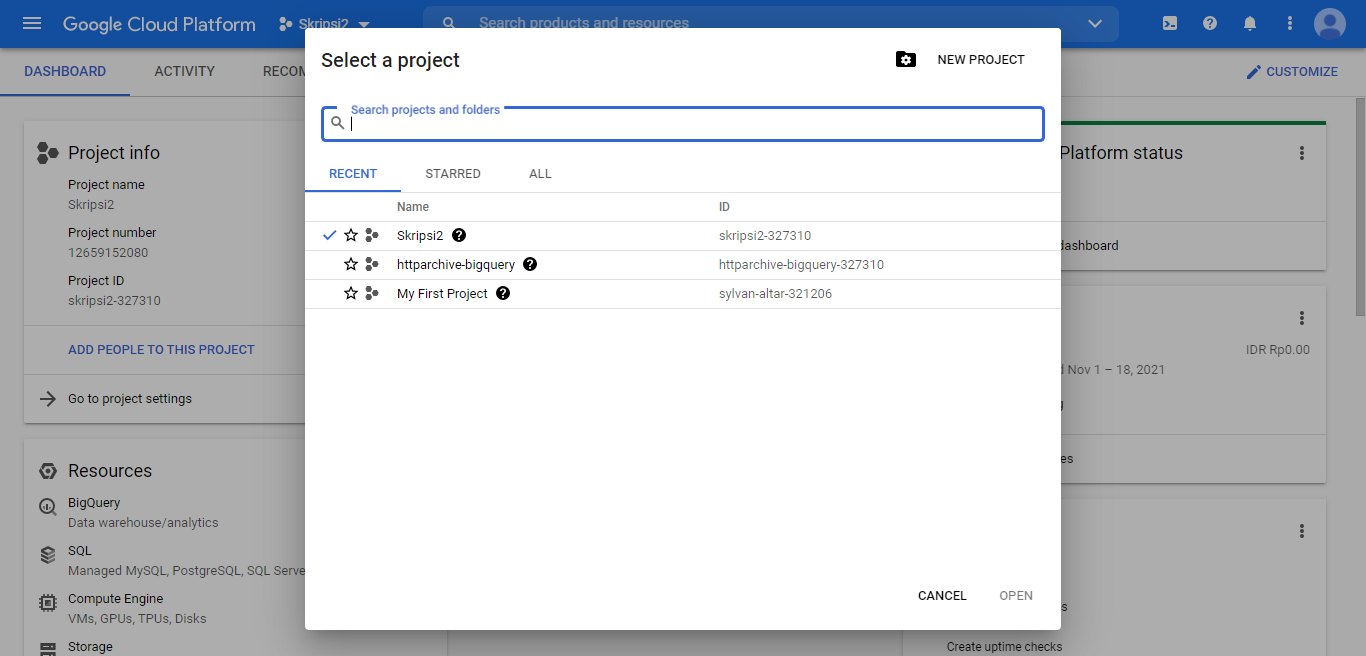
\includegraphics[scale=0.5]{Gambar/pilih_project.PNG}  
		\caption{Create atau Open Project} 
		\label{fig:create_or_open} 
	\end{figure}
	\item Membuka \textit{console} kemudian memilih BigQuery.
	\begin{figure}[H]
		\centering  
		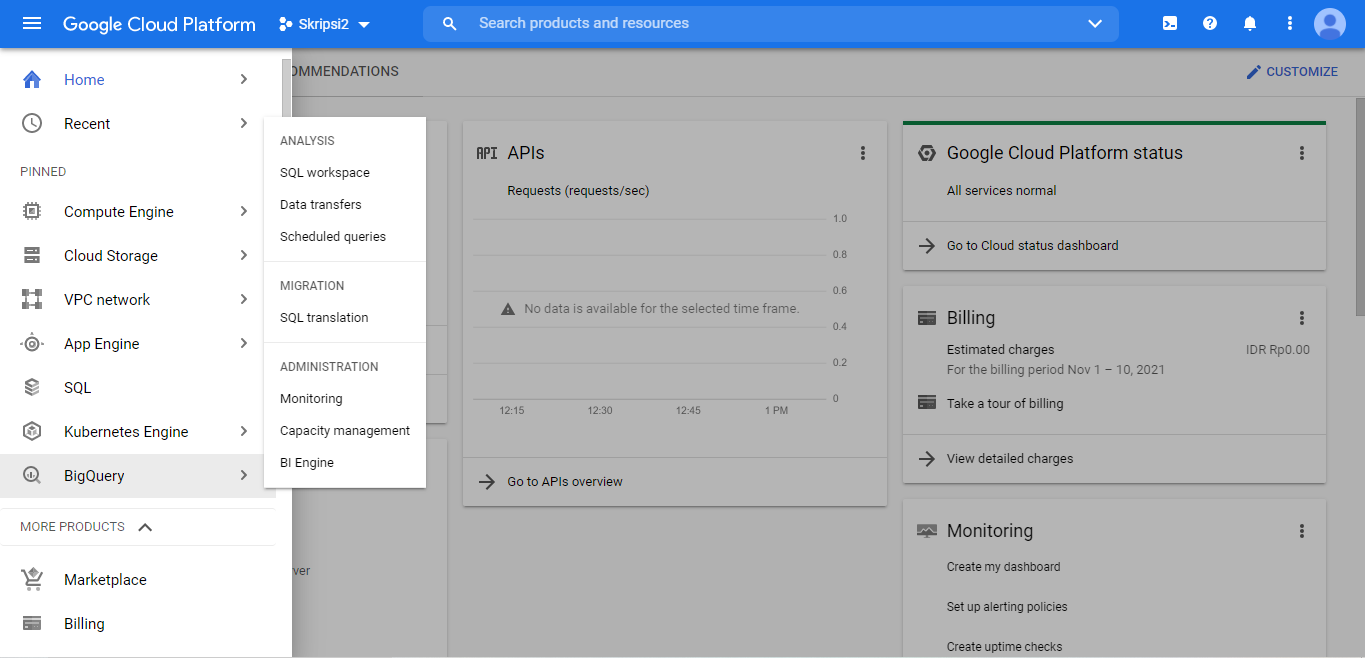
\includegraphics[scale=0.5]{Gambar/console_BigQuery.PNG}  
		\caption{Membuka BigQuery} 
		\label{fig:BQ} 
	\end{figure}
	\item Pada tab explorer terdapat project kemudian pengguna harus menekan tombol titik tiga dan piliih \textit{create} dataset.
	\begin{figure}[H]
		\centering  
		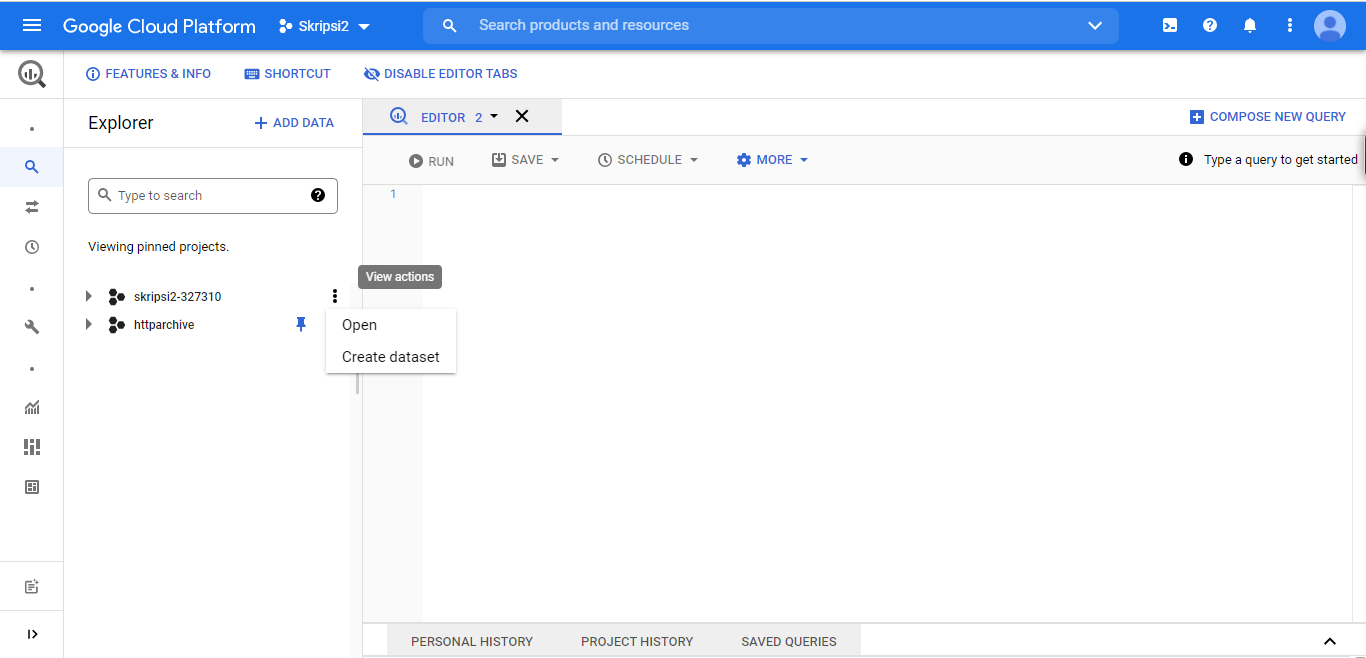
\includegraphics[scale=0.5]{Gambar/create_dataset.PNG}  
		\caption{Membuat Dataset Baru} 
		\label{fig:creat_dataset} 
	\end{figure}
	\item Buka dataset, kemudian pilih menu \textit{create table}.
	\begin{figure}[H]
		\centering  
		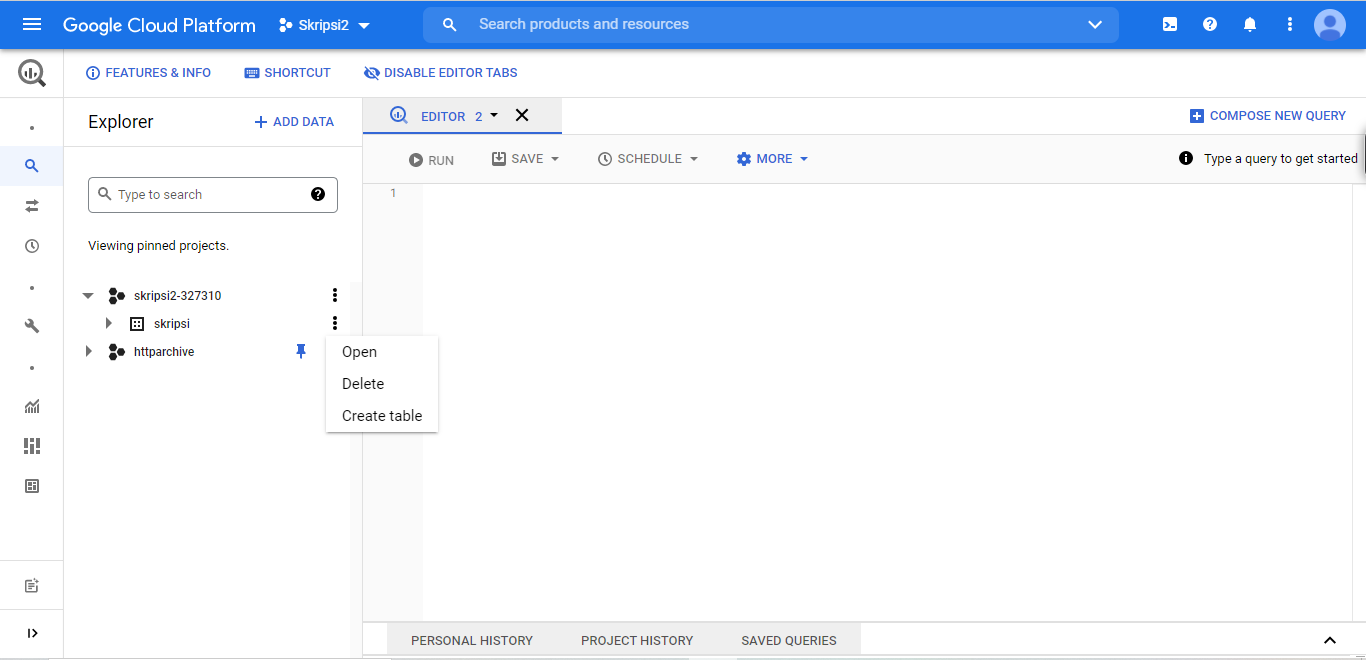
\includegraphics[scale=0.5]{Gambar/create_table.PNG}  
		\caption{Membuat Tabel Baru} 
		\label{fig:create_table} 
	\end{figure}
\end{enumerate}

\subsection{ReactJS}
Selain penggunaan BigQuery, skripsi ini juga menggunakan ReactJS dalam pembuatan charts maupun melakukan perbandingan versi dari aplikasi. Data yang dipakai untuk membuat chart merupakan data JSON yang sudah di-\textit{download} melalui BigQuery. Pembuatan project react dapat dilakukan dengan menggunakan sintaks:
\begin{verbatim}
	npx create-react-app my-app
	cd my-app
	npm start
\end{verbatim}

\section{Dataset Pada HTTP Archive}
Di dalam HTTP Archive terdapat dataset yang dapat diambil menggunakan teknologi BigQuery, dataset tersebut adalah sebagai berikut:
\begin{enumerate}
	\item almanac\\
	Pada tabel ini tidak terdapat keterangan dan tidak berhubungan dengan skripsi ini.
	\item blink$\_$features\\
	Pada tabel ini tidak terdapat keterangan dan tidak berhubungan dengan skripsi ini.
	\item core$\_$web$\_$vitals\\
	Pada tabel ini tidak terdapat keterangan dan tidak berhubungan dengan skripsi ini.
	\item latest\\
	Pada tabel ini tidak terdapat keterangan dan tidak berhubungan dengan skripsi ini.
	\item lighthouse\\
	Dataset pada lighthouse berisi tabel-tabel dari bulan Juni tahun 2017 sampai dengan sekarang yang terdiri dari website pada mobile. Dataset bulan Agustus tahun 2020 baris pada mobile memiliki 6.290.147 baris \ref{table:ct_lh_mobile} yang dapat dianalisis. Masing-masing terdiri dari URL dan report. \textit{URL (Uniform Resource Locator)} merupakan nama-nama domain dan \textit{report}. Tetapi tabel ini tidak digunakan dalam pengerjaan skripsi ini. 
	
	
	\begin{table}[H]
		\centering
		\begin{tabular*}{\textwidth}{|l|p{14.4cm}|}
			\hline
			\textbf{url} & \url{https://votesearch.utah.gov/}\\ 
			\hline
			\textbf{report} & \{"userAgent":"Mozilla/5.0 (X11; Linux x86\_64) AppleWebKit/537.36 (KHTML, like Gecko) Chrome/84.0.4147.105 Safari/537.36","environment":\{"networkUserAgent": "Mozilla/5.0 (Linux; Android 7.0; Moto G (4)) AppleWebKit/537.36 (KHTML, like Gecko) Chrome/84.0.4143.7 Mobile Safari/537.36 Chrome-Lighthouse","hostUserAgent":"Mozilla/5.0 (X11; Linux x86\_64) AppleWebKit/537.36 (KHTML, like Gecko) Chrome/84.0.4147.105 Safari/537.36","benchmarkIndex":506\},"lighthouseVersion": "6.1.1" ,"fetchTime": "2020-08-06T10:36:03.335Z" ,"requestedUrl":"\url{https://votesearch.utah.gov/}","finalUrl":"\url{https://vote.utah.gov/}","runWarnings":["The page may not be loading as expected because your test URL (\url{https://votesearch.utah.gov/}) was redirected to https://vote.utah.gov/. Try testing the second URL directly."],"audits":\{"is-on-https":\{"id":"is-on-https","title":"Does not use HTTPS","description":"All sites should be protected with HTTPS, even ones that don't handle sensitive data. This includes avoiding [mixed content](\url{https://developers.google.com}...\\
			\hline
			
		\end{tabular*}
		\caption{Lighthouse Data Example}
		\label{table:ct_lh_mobile}
	\end{table}
	
	% \begin{sidewaystable} % <-- HERE
		% \centering
		% \begin{tabular}{|l|l|@{\extracolsep{\fill}}p{18cm}|}\hline
			% 1 & \url{https://votesearch.utah.gov/} & \{"userAgent":"Mozilla/5.0 (X11; Linux x86\_64) AppleWebKit/537.36 (KHTML, like Gecko) Chrome/84.0.4147.105 Safari/537.36","environment":\{"networkUserAgent": "Mozilla/5.0 (Linux; Android 7.0; Moto G (4)) AppleWebKit/537.36 (KHTML, like Gecko) Chrome/84.0.4143.7 Mobile Safari/537.36 Chrome-Lighthouse","hostUserAgent":"Mozilla/5.0 (X11; Linux x86\_64) AppleWebKit/537.36 (KHTML, like Gecko) Chrome/84.0.4147.105 Safari/537.36","benchmarkIndex":506\},"lighthouseVersion": "6.1.1" ,"fetchTime": "2020-08-06T10:36:03.335Z" ,"requestedUrl":"\url{https://votesearch.utah.gov/}","finalUrl":"\url{https://vote.utah.gov/}","runWarnings":["The page may not be loading as expected because your test URL (\url{https://votesearch.utah.gov/}) was redirected to https://vote.utah.gov/. Try testing the second URL directly."],"audits":\{"is-on-https":\{"id":"is-on-https","title":"Does not use HTTPS","description":"All sites should be protected with HTTPS, even ones that don't handle sensitive data. This includes avoiding [mixed content](\url{https://developers.google.com}...\\
			% \hline
			% \end{tabular}
		% \caption{Lighthouse Data Example}
		% \label{table:ct_lh_mobile}
		% \end{sidewaystable} % <-- HERE
	
	
	%     \begin{table}[H]
		% \centering
		% \begin{tabular*}{\textwidth}{|l|l|@{\extracolsep{\fill}}p{8.8cm}|}
			%  \hline
			%  \textbf{Row} & \textbf{url} & \textbf{report}\\
			%  \hline
			% 1 & \url{https://votesearch.utah.gov/} & \{"userAgent":"Mozilla/5.0 (X11; Linux x86\_64) AppleWebKit/537.36 (KHTML, like Gecko) Chrome/84.0.4147.105 Safari/537.36","environment":\{"networkUserAgent": "Mozilla/5.0 (Linux; Android 7.0; Moto G (4)) AppleWebKit/537.36 (KHTML, like Gecko) Chrome/84.0.4143.7 Mobile Safari/537.36 Chrome-Lighthouse","hostUserAgent":"Mozilla/5.0 (X11; Linux x86\_64) AppleWebKit/537.36 (KHTML, like Gecko) Chrome/84.0.4147.105 Safari/537.36","benchmarkIndex":506\},"lighthouseVersion": "6.1.1" ,"fetchTime": "2020-08-06T10:36:03.335Z" ,"requestedUrl":"\url{https://votesearch.utah.gov/}","finalUrl":"\url{https://vote.utah.gov/}","runWarnings":["The page may not be loading as expected because your test URL (\url{https://votesearch.utah.gov/}) was redirected to https://vote.utah.gov/. Try testing the second URL directly."],"audits":\{"is-on-https":\{"id":"is-on-https","title":"Does not use HTTPS","description":"All sites should be protected with HTTPS, even ones that don't handle sensitive data. This includes avoiding [mixed content](\url{https://developers.google.com}...\\
			% \hline
			% 2 & \url{https://otricolore.ru/} & \{"userAgent": "Mozilla/5.0 (X11; Linux x86\_64) AppleWebKit/537.36 (KHTML, like Gecko) Chrome/84.0.4147.125 Safari/537.36","environment":\{"networkUserAgent": "Mozilla/5.0 (Linux; Android 7.0; Moto G (4)) AppleWebKit/537.36 (KHTML, like Gecko) Chrome/84.0.4143.7 Mobile Safari/537.36 Chrome-Lighthouse","hostUserAgent": "Mozilla/5.0 (X11; Linux x86\_64) AppleWebKit/537.36 (KHTML, like Gecko) Chrome/84.0.4147.125 Safari/537.36","benchmarkIndex":456},"lighthouseVersion": "6.2.0" ,"fetchTime":"2020-08-11T09:30:51.743Z", "requestedUrl": "\url{https://otricolore.ru/}", "finalUrl": "\url{https://otricolore.ru/}","runWarnings":[],"audits":\{"is-on-https":\{"id":"is-on-https","title":"Uses HTTPS","description":"All sites should be protected with HTTPS, even ones that don't handle sensitive data. This includes avoiding [mixed content](\url{https://developers.google.com/web/fundamentals/security/prevent-mixed-content/what-is-mixed-content}), where some resources are loaded over HTTP despite the initial request being servedover HTTPS. HTTPS prevents int…\\
		% \hline
		% \end{tabular*}
	% \caption{Lighthouse Data Example}
	% \label{table:ct_lh_mobile}
	% \end{table}

\item pages\\
Dataset pada pages berisi tabel-tabel dari bulan Januari tahun 2016 sampai dengan sekarang yang terdiri dari website pada desktop dan mobile. Dataset bulan Agustus tahun 2020 baris pada desktop memiliki 5.593.642 baris dan pada mobile memiliki 6.347.640 baris. Contoh data dapat dilihat pada tabel \ref{table:pages_data_sample}.
Masing-masing terdiri dari URL dan payload. \textit{URL (Uniform Resource Locator)} merupakan nama-nama domain dan \textit{payload}. Tetapi tabel ini tidak digunakan dalam pengerjaan skripsi ini.

\begin{table}[H]
	\centering
	\begin{tabular*}{\textwidth}{|l|p{14.13cm}|}
		\hline
		\textbf{url} & \url{https://tutorinmobiliario.cl/}\\ 
		\hline
		\textbf{payload} & \{"startedDateTime":"2020-08-14T17:45:37.606+00:00", "title": "Run 1, First View for \url{https://tutorinmobiliario.cl/}", "id": "page\_1\_0\_1", "pageTimings": \{"onLoad":27048,"onContentLoad":-1, "\_startRender":6500\}, "\_cpu.BlinkGC.LazySweepInIdle":10, "\_testStartOffset":0,"\_start\_epoch":0, "\_cpu.ParseAuthorStyleSheet":95,"\_bytesOutDoc": 208779, "\_cpu.V8.GC\_MC\_CLEAR\_STRING\_TABLE":1, "\_cpu.V8.GC\_SCAVENGER\_SCAVENGE\_UPDATE \_REFS": 0, "\_cpu.V8.GC\_MC\_MARK\_EMBEDDER\_TRACING\_CLOSURE":0, "\_cpu.V8.GC\_MC\_MARK\_FINISH\_INCREMENTAL": 0, "\_firstPaint":6445.524999995541, "\_cpu.BlinkGC.AtomicPauseMarkEpilogue":0,  "\_cpu.V8.GC\_MC\_INCREMENTAL\_EMBEDDER \_PROLOGUE":7, "\_cpu.V8.GC\_SCAVENGER\_COMPLETE\_SWEEP\_ARRAY\_BUFFERS":0, "\_cpu.V8.GC\_MC\_EVACUATE\_REBALANCE":0,"\_optimization\_checked":1, "\_cpu.V8.GC\_MC\_MARK\_ROOTS":0, "\_cpu.BlinkGC. IncrementalMarkingStartMarking": 4, "\_responses\_404":0, "\_URL": "\url{https://tutorinmobiliario.cl/}", "\_cpu.V8.GC\_SCAVENGER\_SCAVENGE\_ROOTS":3, "\_loadEventStart":27048, "\_cpu.EvaluateScript":452 , "\_score\_gzip":100, "\_cpu.V8.GC\_MC\_MARK\_WEAK\_CLOSURE\_EPHEMERON\_…\\
		\hline
		
	\end{tabular*}
	\caption{Pages Data Example}
	\label{table:pages_data_sample}
\end{table}

%     \begin{sidewaystable} % <-- HERE
	% \centering
	% \begin{tabular}{|l|l|@{\extracolsep{\fill}}p{18cm}|}\hline
		% 1 & https://tutorinmobiliario.cl/ & \{"startedDateTime":"2020-08-14T17:45:37.606+00:00", "title": "Run 1, First View for \url{https://tutorinmobiliario.cl/}", "id": "page\_1\_0\_1", "pageTimings": \{"onLoad":27048,"onContentLoad":-1, "\_startRender":6500\}, "\_cpu.BlinkGC.LazySweepInIdle":10, "\_testStartOffset":0,"\_start\_epoch":0, "\_cpu.ParseAuthorStyleSheet":95,"\_bytesOutDoc": 208779, "\_cpu.V8.GC\_MC\_CLEAR\_STRING\_TABLE":1, "\_cpu.V8.GC\_SCAVENGER\_SCAVENGE\_UPDATE \_REFS": 0, "\_cpu.V8.GC\_MC\_MARK\_EMBEDDER\_TRACING\_CLOSURE":0, "\_cpu.V8.GC\_MC\_MARK\_FINISH\_INCREMENTAL": 0, "\_firstPaint":6445.524999995541, "\_cpu.BlinkGC.AtomicPauseMarkEpilogue":0,  "\_cpu.V8.GC\_MC\_INCREMENTAL\_EMBEDDER \_PROLOGUE":7, "\_cpu.V8.GC\_SCAVENGER\_COMPLETE\_SWEEP\_ARRAY\_BUFFERS":0, "\_cpu.V8.GC\_MC\_EVACUATE\_REBALANCE":0,"\_optimization\_checked":1, "\_cpu.V8.GC\_MC\_MARK\_ROOTS":0, "\_cpu.BlinkGC.IncrementalMarkingStartMarking":4, "\_responses\_404":0, "\_URL": "https://tutorinmobiliario.cl/", "\_cpu.V8.GC\_SCAVENGER\_SCAVENGE\_ROOTS":3, "\_loadEventStart":27048, "\_cpu.EvaluateScript":452 , "\_score\_gzip":100, "\_cpu.V8.GC\_MC\_MARK\_WEAK\_CLOSURE\_EPHEMERON\_…\\
		% \hline
		% \end{tabular}
	% \caption{Pages Data Sample}
	% \label{table:pages_data_sample}
	% \end{sidewaystable} % <-- HERE

%     \begin{table}[H]
	% \centering
	% \begin{tabular*}{\textwidth}{|l|l|@{\extracolsep{\fill}}p{8.8cm}|}
		%  \hline
		%  \textbf{Row} & \textbf{url} & \textbf{payload}\\
		%  \hline
		% 1 & https://tutorinmobiliario.cl/ & \{"startedDateTime":"2020-08-14T17:45:37.606+00:00", "title": "Run 1, First View for \url{https://tutorinmobiliario.cl/}", "id": "page\_1\_0\_1", "pageTimings": \{"onLoad":27048,"onContentLoad":-1, "\_startRender":6500\}, "\_cpu.BlinkGC.LazySweepInIdle":10, "\_testStartOffset":0,"\_start\_epoch":0, "\_cpu.ParseAuthorStyleSheet":95,"\_bytesOutDoc": 208779, "\_cpu.V8.GC\_MC\_CLEAR\_STRING\_TABLE":1, "\_cpu.V8.GC\_SCAVENGER\_SCAVENGE\_UPDATE\_REFS": 0, "\_cpu.V8.GC\_MC\_MARK\_EMBEDDER\_TRACING\_CLOSURE":0, "\_cpu.V8.GC\_MC\_MARK\_FINISH\_INCREMENTAL": 0, "\_firstPaint":6445.524999995541, "\_cpu.BlinkGC.AtomicPauseMarkEpilogue":0,  "\_cpu.V8.GC\_MC\_INCREMENTAL\_EMBEDDER\_PROLOGUE":7, "\_cpu.V8.GC\_SCAVENGER\_COMPLETE\_SWEEP\_ARRAY\_BUFFERS":0, "\_cpu.V8.GC\_MC\_EVACUATE\_REBALANCE":0,"\_optimization\_checked":1, "\_cpu.V8.GC\_MC\_MARK\_ROOTS":0, "\_cpu.BlinkGC.IncrementalMarkingStartMarking":4, "\_responses\_404":0, "\_URL": "https://tutorinmobiliario.cl/", "\_cpu.V8.GC\_SCAVENGER\_SCAVENGE\_ROOTS":3, "\_loadEventStart":27048, "\_cpu.EvaluateScript":452 , "\_score\_gzip":100, "\_cpu.V8.GC\_MC\_MARK\_WEAK\_CLOSURE\_EPHEMERON\_…\\
		% \hline
		% 2 & https://nishinatoshiharu.com/ & \{"startedDateTime":"2020-08-18T21:50:57.272+00:00","title":"Run 1, First View for https://nishinatoshiharu.com/","id":"page$\_$1$\_$0$\_$1","pageTimings":\{"onLoad":24788,"onContentLoad":-1,"$\_$startRender":4800\},"$\_$cpu.BlinkGC.LazySweepInIdle":28,"$\_$testStartOffset":0,"$\_$start$\_$epoch":0,"$\_$cpu.ParseAuthorStyleSheet":98,"$\_$bytesOutDoc":469240,"$\_$cpu.V8.GC$\_$MC$\_$CLEAR$\_$STRING$\_$TABLE":1,"$\_$cpu.V8.GC$\_$SCAVENGER$\_$SCAVENGE$\_$UPDATE$\_$REFS":0,"$\_$cpu.V8.GC$\_$MC$\_$MARK$\_$EMBEDDER$\_$TRACING$\_$CLOSURE":0,"$\_$cpu.V8.GC$\_$MC$\_$MARK$\_$FINISH$\_$INCREMENTAL":0,"$\_$firstPaint":4826.009999997041,"$\_$cpu.BlinkGC.AtomicPauseMarkEpilogue":0,"$\_$cpu.V8.GC$\_$MC$\_$INCREMENTAL$\_$EMBEDDER$\_$PROLOGUE":14,"$\_$cpu.V8.GC$\_$SCAVENGER$\_$COMPLETE$\_$SWEEP$\_$ARRAY$\_$BUFFERS":0,"$\_$cpu.V8.GC$\_$MC$\_$EVACUATE$\_$REBALANCE":0,"$\_$optimization$\_$checked":1,"$\_$cpu.V8.GC$\_$MC$\_$MARK$\_$ROOTS":0,"$\_$cpu.BlinkGC.IncrementalMarkingStartMarking":9,"$\_$responses$\_$404":0,"$\_$URL":"https://nishinatoshiharu.com/","$\_$cpu.V8.GC$\_$SCAVENGER$\_$SCAVENGE$\_$ROOTS":5,"$\_$loadEventStart":24788,"$\_$cpu.EvaluateScript":712,"$\_$score$\_$gzip":100,"$\_$cpu.V8.GC$\_$MC$\_$MARK$\_$WEAK$\_$CLOSURE$\_$EPHEMERON…\\
		% \hline
		% \end{tabular*}
	% \caption{Pages Data Sample}
	% \label{table:pages_data_sample}
	% \end{table}


\item requests\\
Dataset pada request berisi tabel-tabel dari bulan Januari tahun 2016 sampai dengan sekarang yang terdiri dari website pada desktop dan mobile. Dataset bulan Agustus tahun 2020 baris pada desktop memiliki 535.841.778 baris dan pada mobile memiliki 579.752.745 baris yang dapat dianalisis. Masing-masing terdiri dari URL dan payload. \textit{URL (Uniform Resource Locator)} merupakan nama-nama domain dan \textit{payload}. Tetapi tabel ini tidak digunakan dalam pengerjaan skripsi ini.
\item response$\_$bodies\\
Dataset pada response$\_$bodies berisi tabel-tabel dari bulan Januari tahun 2016 sampai dengan sekarang yang terdiri dari website pada desktop dan mobile. Dataset bulan Agustus tahun 2020 baris pada desktop memiliki 215.621.667 baris dan pada mobile memiliki 270.249.686 baris yang dapat dianalisis. Masing-masing terdiri dari page, URL, body, truncated, dan requestId. Tetapi tabel ini tidak digunakan dalam pengerjaan skripsi ini.
\item sample$\_$data\\
Pada tabel ini tidak terdapat keterangan dan tidak berhubungan dengan skripsi ini.
\item sample$\_$data$\_$2020\\
Pada tabel ini tidak terdapat keterangan dan tidak berhubungan dengan skripsi ini.
\item scratchspace\\
Pada tabel ini tidak terdapat keterangan dan tidak berhubungan dengan skripsi ini.
\item summary$\_$pages\\
Dataset pada summary$\_$pages berisi tabel-tabel dari bulan November tahun 2010 sampai dengan sekarang yang terdiri dari website pada desktop dan mobile. Dataset bulan Agustus tahun 2020 baris pada desktop memiliki 5.593.642 baris dan pada mobile memiliki 6.347.919 baris yang dapat dianalisis. Masing-masing terdiri dari pageid, createDate, archive, label, crawlid, wptid, wptrun, url, urlShort, urlhash, cdn, startedDateTime, TTFB, renderStart, onContentLoaded, onLoad, fullyLoad, visualComplete, PageSpeed, SpeedIndex, rank, reqTotal, reqHTML, reqJS, reqCSS, reqImg, reqGif, reqJpg, reqPng, reqFont, reqFlash, reqJson, reqOther, bytesTotal, bytesHTML, bytesJS, bytesCSS, bytesImg, bytesGif, bytesJpg, bytesPng, bytesFont, bytesFlash, bytesJson, bytesOther, bytesHtmlDoc, numDomains, maxDomainReqs, numRedirects, numErrors, numGlibs, numHttps, numCompressed, numDomElements, maxageNull, maxage0, maxage1, maxage30, maxage365, maxageMore, gzipTotal, gzipSavings, $\_$connections, $\_$adult$\_$site, avg$\_$dom$\_$depth, document$\_$height, document$\_$width, localstorage$\_$size, sessionstorage$\_$size, num$\_$iframes, num$\_$scripts, doctype, meta$\_$viewport, reqAudio, reqVideo, reqText, reqXml, reqWebp, reqSvg, bytesAudio, bytesVideo, bytesText, bytesXml, bytesWebp, bytesSvg, num$\_$scripts$\_$async, num$\_$scripts$\_$sync, usertiming. Tetapi tabel ini tidak digunakan dalam pengerjaan skripsi ini.
\item summary$\_$requests\\
Dataset pada response$\_$requests berisi tabel-tabel dari bulan November tahun 2010 sampai dengan sekarang yang terdiri dari website pada desktop. Dataset bulan Agustus tahun 2020 baris pada desktop memiliki 215.621.667 baris dan pada mobile memiliki 1.234.599 baris yang dapat dianalisis. Masing-masing terdiri dari requestid, pageid, startedDateTime, time, method, url, urlShort, redirectUrl, firstReq, firstHtml, reqHttpVersion, reqHeaderSize, reqBodySize, reqCookieLen, reqOtherHeader, status, respHttpVersion, respHeaderSize, respBodySize, respSize, respCookieLen, expAge, mimeType, respOtherHeader, req$\_$accept, req$\_$accept$\_$charset, req$\_$accept$\_$encoding, req$\_$accept$\_$language, req$\_$connection, req$\_$host, req$\_$if$\_$modified$\_$since, req$\_$if$\_$none$\_$match, req$\_$referer, req$\_$user$\_$agent, resp$\_$accept$\_$ranges, resp$\_$age, resp$\_$cache$\_$control, resp$\_$connection, resp$\_$content$\_$encoding, resp$\_$content$\_$language, resp$\_$content$\_$length, resp$\_$content$\_$location, resp$\_$content$\_$type, resp$\_$date, resp$\_$etag, resp$\_$expires, resp$\_$keep$\_$alive, resp$\_$last$\_$modified, resp$\_$location, resp$\_$pragma, resp$\_$server, resp$\_$transfer$\_$encoding, resp$\_$vary, resp$\_$via, resp$\_$x$\_$powered$\_$by. Tetapi tabel ini tidak digunakan dalam pengerjaan skripsi ini.
\item technologies\\
Dataset pada technologies berisi tabel-tabel dari bulan Januari tahun 2016 sampai dengan sekarang yang terdiri dari website pada desktop dan mobile. Dataset bulan Agustus tahun 2020 baris pada desktop memiliki 61.203.638 baris  dapat dilihat pada gambar \ref{table:ct_tech_desktop} dan pada mobile memiliki 67.452.994 baris \ref{table:ct_tech_mobile} yang dapat dianalisis. Masing-masing terdiri dari 4 kolom yaitu \textit{URL}, \textit{category}, \textit{app}, \textit{info}. Pada kolom \textit{URL (Uniform Resource Locator)} merupakan nama-nama domain, \textit{category} merupakan jenis aplikasi yang digunakan pada website tersebut, \textit{app} merupakan aplikasi yang digunakan website tersebut, \textit{info} merupakan informasi tambahan dari aplikasi. 

\begin{table}[H]
	\centering
	\begin{tabular}{|l|l|p{3cm}|p{3cm}|l|}
		\hline
		\textbf{Row} & \textbf{url} & \textbf{category} & app & info\\
		\hline
		1 & https://www.3-king.com/ & Analytics & Google Analytics & \\
		\hline
		2 & https://www.fleabites.net/ & Miscellaneous & Twitter Emoji (Twemoji) & \\
		\hline
		3 & http://www.elcarnicero.cl/ & Widgets & OWL Carousel & \\
		\hline
		4 & https://thankyou.ws/ & Analytics & Google Analytics & \\
		\hline
		5 & https://rogerwaters.com/ & Reverse proxies & Nginx & \\
		\hline
		6 & http://www.palaciodaslampadas.com.br/ & JavaScript libraries & jQuery & 2.1.1\\
		\hline
		7 & https://copenhagencamping.dk/ & CMS & WordPress & \\
		\hline
		8 & https://eachat.ma/ & Ecommerce & WooCommerce & 4.3.0\\
		\hline
		9 & https://advokat-bondarchuk.ru/ & Blogs & WordPress & \\
		\hline
		10 & https://passport.rsl.ru/ & JavaScript libraries & jQuery & 1.7.1\\
		\hline
	\end{tabular}
	\caption{Technologies Desktop Data Sample}
	\label{table:ct_tech_desktop}
\end{table}

\begin{table}[H]
	\centering
	\begin{tabular}{|l|l|p{3cm}|p{3cm}|l|}
		\hline
		\textbf{Row} & \textbf{url} & \textbf{category} & app & info\\
		\hline
		1 & http://www.carobd.fr/ & UI frameworks & Bootstrap & 4.1.3\\
		\hline
		2 & http://www.minikabebe.com/ & Font scripts & Font Awesome & \\
		\hline
		3 & https://sibirskisamojedcom.wordpress.com/ & Blogs & WordPress & \\
		\hline
		4 & https://www.peauideale.com/ & Analytics & Google Analytics & \\
		\hline
		5 & https://www.bestcours.com/ & JavaScript libraries & jQuery & 1.11.1\\
		\hline
		6 & https://www.chirurgo-stefanoenrico.it/ & UI frameworks & Bootstrap & \\
		\hline
		7 & https://retrocores.com/ & JavaScript libraries & jQuery & 1.12.4\\
		\hline
		8 & https://pakmule.com/ & Web servers & Apache & \\
		\hline
		9 & https://edilsonalves.com.br/ & JavaScript libraries & jQuery & 1.12.4\\
		\hline
		10 & https://mobilierdasie.com/ & Ecommerce & Google Analytics Enhanced eCommerce & \\
		\hline
	\end{tabular}
	\caption{Technologies Mobile Data Sample}
	\label{table:ct_tech_mobile}
\end{table}


\item urls\\
Pada tabel ini tidak terdapat keterangan dan tidak berhubungan dengan skripsi ini.
\item wappalyzer\\
Pada tabel ini tidak terdapat keterangan dan tidak berhubungan dengan skripsi ini.
\end{enumerate}

\section{Langkah-Langkah Query Yang Dilakukan}
Pada section ini akan dijelaskan tentang langkah-langkah query yang dilakukan dalam memperoleh data dan analisis yang dilakukan. Data yang diambil adalah data percobaan sebanyak 100 data. Data yang diambil merupakan dataset dari tabel technologies 2020$\_$08$\_$01:

\subsection{Mengumpulkan List Website}
Langkah pertama yang dilakukan yaitu mengumpulkan website. Website yang dicari tidak berdasarkan berdasarkan \textit{rank} karena tidak tersedia pada dataset tersebut. Berikut adalah \textit{query} yang digunakan untuk mengumpulkan list website.
\begin{verbatim}
SELECT url
FROM `httparchive.technologies.2020_08_01_*`
ORDER BY url asc
LIMIT 100
\end{verbatim}

\subsection{Mencari Aplikasi Yang Digunakan Website}
Setiap website akan dicari aplikasi apa saja yang digunakan dalam pembangunan website tersebut dan versi dari aplikasi yang dipakainya. Berikut adalah query yang digunakan.
\begin{verbatim}
SELECT url, app, info
FROM `httparchive.technologies.2020_08_01_*`
ORDER BY url asc
LIMIT 100
\end{verbatim}

\subsection{Mengelompokkan Berdasarkan Nama Semua Aplikasi Yang Dipakai}
Pengelompokan aplikasi dapat dilakukan dengan menggunakan query. Berikut adalah query yang digunakan.
\begin{verbatim}
SELECT tabelName.app, num.num_sites , versioned.versioned_count , unversioned.unversioned_count
FROM 
(SELECT DISTINCT app
FROM `httparchive.technologies.2020_08_01_*` ) tabelName

LEFT JOIN 

(SELECT tabel1.app, count(app) AS versioned_count
FROM `httparchive.technologies.2020_08_01_*` AS tabel1
WHERE tabel1.app!="" AND tabel1.info != "" 
GROUP BY tabel1.app) AS versioned

ON(versioned.app = tabelName.app)

LEFT JOIN

(SELECT tabel2.app, count(app) AS unversioned_count
FROM `httparchive.technologies.2020_08_01_*` AS tabel2
WHERE tabel2.app!="" AND tabel2.info = "" 
GROUP BY tabel2.app) AS unversioned

ON (unversioned.app = tabelName.app)

LEFT JOIN 

(SELECT app, count(url) AS num_sites
FROM `httparchive.technologies.2020_08_01_*`
GROUP BY app) AS num

ON (tabelName.app = num.app)
LIMIT 100
\end{verbatim}

\subsection{Mencari Data Tentang Versi Aplikasi Yang Masih Didukung}
Sebelum menentukan suatau aplikasi usang atau tidak, kita harus mencari versi dari setiap aplikasi secara manual. Versi setiap aplikasi dapat dilihat di-\textit{official documentation} dari setiap aplikasi. Hasil pencarian dari aplikasi yang masih didukung dapat dilihat pada gambar \ref{appData}. 

\subsection{Melakukan Perbandingan Antara Versi Aplikasi Yang Masih Dipakai Sekarang Dengan Versi Aplikasi Yang Masih Didukung}




\section{Hasil Sample Data Dengan Beberapa Aplikasi}
Diambil 29 data sample dengan aplikasi dan nomor versinya. Pada gambar \ref{fig:data_sample_res} aplikasi Lodash dengan versi 4.7.15 memiliki jumlah 265.552 kali dipakai oleh website.
\begin{figure}[H]
\centering  
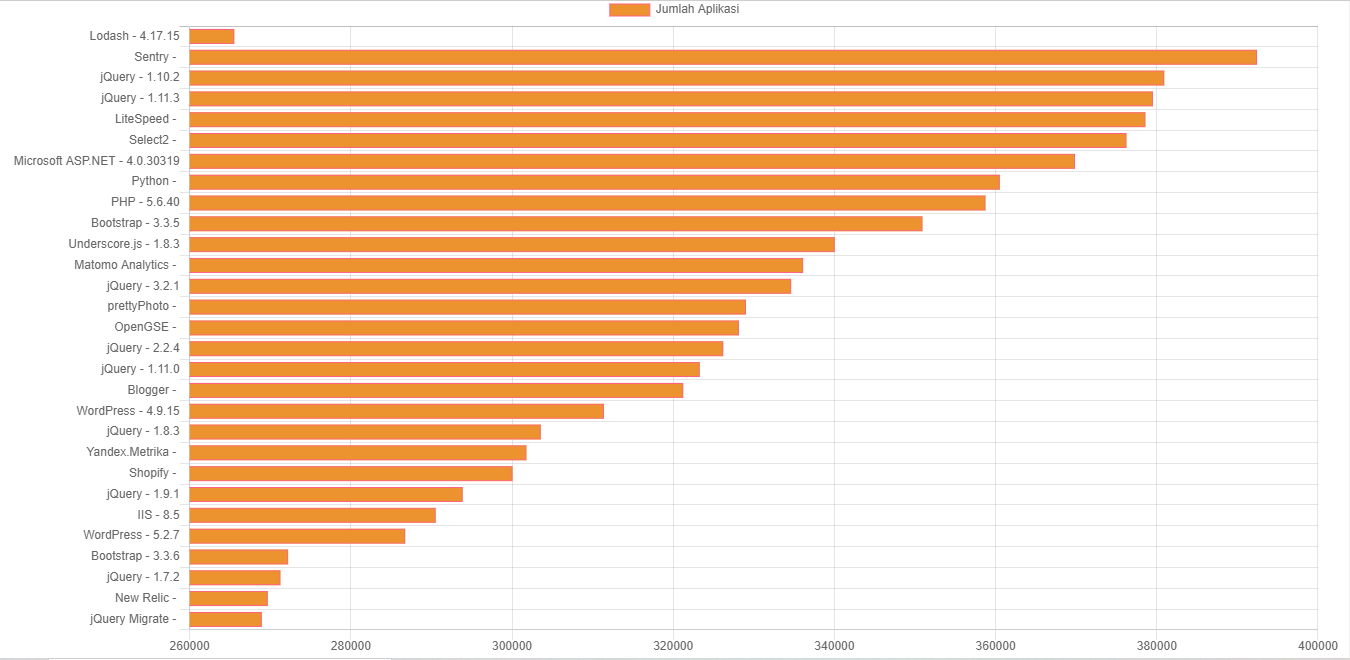
\includegraphics[scale=0.5]{Gambar/hasil_chart_all.PNG}  
\caption{Data Sample Jumlah Aplikasi Dengan Versi yang Dipakai} 
\label{fig:data_sample_res} 
\end{figure}